% This is the chapter 'Modeling' to the "Hodgkin-Huxley neuron model V2.0 book"
% Last edited 2026.08.08


\chapter[Rugalmas modell]{Rugalmas modell\label{ch:VModel-Elastic}}

\iflatexml
\else
\minitoc
\fi


A neuront úgy vezettük be, hogy az egy vizes oldattal töltött
lipid gömböcske, ami tranziens állapotban csillapított rezgőmozgást végez, és természetesen a benne található vizes 
oldatot is rezgeti. Modellünkben egy rugalmas alaplappal ellátott
tartályban az alapra ható erőlökéssel rezgést indítunk el,
ami gyorsan lecsillapodik. Önmagában ez a modell tisztán a mechanika 
diszciplinájához tartozik. A neuron esetében a vizes oldat
ionokat tartalmaz, és a vibráló folyadékban levő kis mennyiségű
ion is rezgőmozgást végez, azaz feszültséghullámot generál,
bár az oda-vissza mozgó ionok miatt csupán minimális anyagtranszporttal jár.

The mechanical (elastic) model takes us one step closer to the correct model: it is a forerunner of the unified model. It assumes that the action potential is basically generated by the shock wave generated by the elastic membrane, which is significantly distorted by the electrostatic repulsion of the ions in the electrolyte.

The rush-in of $Na^+$ ions results in electric, chemical, and elastic gradients, see~\cite{VeghUnifiedCrossdisciplinaryModel:2026}. The final result (shown in Fig.~\ref{fig:DampedOscillation}) is that the membrane vibrates the 
electrolyte (with the cca. $10^{-3}$ part ions inside).
Moreover, the electrostatic repulsion and the concentration gradient of ions provide an offset voltage that triggers an electrical discharge. 
The two processes are superimposed.

\begin{figure}
\centering
	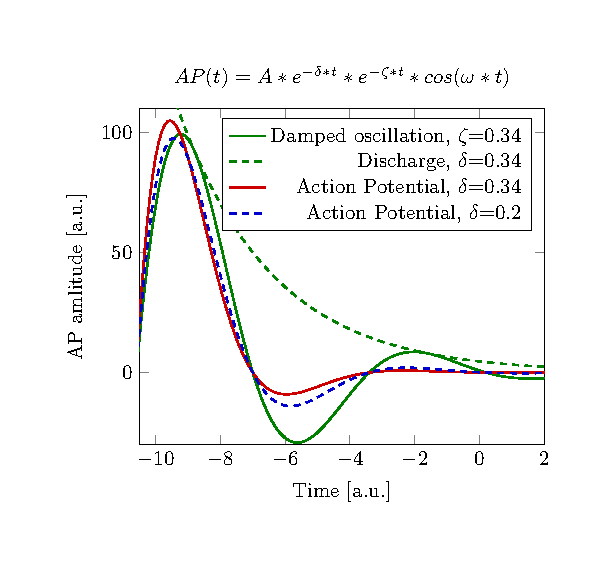
\includegraphics[scale=1.2]{fig/DampedOscillation}
	
	\caption{Describing the generation of an \gls{AP}
		as the superposition of an elastic vibration 
		of the membrane and an electrical discharge process.
		\label{fig:DampedOscillation}}
	
\end{figure}


The sudden rush-in of
$Na^+$ ions has (at least) a double effect. 
One effect is that they press the surface of the membrane that
elastically increases its diameter~\cite{NeuronalDeformation:2020}.
Due to their mutual repulsion,
the ions experience a strong electrical force toward the membrane. It represents an impulse $J=F\,\Delta t$ [N\,s], that enables estimating the time and energy of the 
change the rush-in causes and explains that the energy needed to 
generate an \gls{AP} is suddenly produced electrically, 
and stored temporarily as elastic energy (the neuron produces the required energy in the background, when \gls{ATP} produces ions by hydrolysis under the effect of the electrical field near to membrane); see~\cite{VeghUnifiedCrossdisciplinaryModel:2026}. 
The case is practically identical to
the deformation of an elastic plate induced by the hydrostatic pressure of a water column. Initially, the aluminum plate is suddenly subjected to hydrostatic pressure, and it reaches equilibrium after initial oscillations. The diagram line of the process is shown in the figure
\cite{HydrostaticWaterColumn:2021}, and the method of simulation is discussed in \cite{Hydrostatic_SPHinXsys:2021}. Compare the diagram line to the
gradient in Fig.~\ref{fig:PhysicalProcessesMembrane}, middle inset.

The elastic force is described by the  
\[
F(t) = F_{max}^{elastic}\times e^{-\zeta*t}\times cos(\omega\times t)
\]
\noindent 
formula. The classical model entirely neglects this elastic gradient. However, it is almost four orders of magnitude higher than the electrical and thermodynamic gradients (see Appendix~\ref{sec:Forces}), explaining why the damped elastic oscillation almost perfectly describes 
the time course of the \gls{AP}. However, the elastic force oscillates and decays exponentially, so the dominance of 
the elastic term changes with time.
The electrical model can perfectly describe \gls{AP} since 
the pressure and the electric field are proportional to the number of ions inside a volume.

The other effect is that a large amount of positive charges
appears in the neuron, significantly increasing the membrane's potential. The axon remains on the resting potential, so the potential gradient drives a current.
A discharge process takes place where the amount of charge
inside the neuron exponentially decreases 
\[
F_{electric}(t) = F^{max}_{electric}\times e^{-\delta*t}
\]

The two effects act at the same time, that is
\[
F_{resulting}(t) = F^{max}_{resulting}\times e^{-\delta*t}  \times e^{-\zeta*t}  \times cos(\omega\times t)
\]
(the two exponential factors have physically different reasons,
but they can be contracted mathematically), resulting
an oscillation shown in Fig.~\ref{fig:DampedOscillation}.
This model combines the effects of two distinct disciplines,
but may not be perfect, because of the dual role of ions:
the electric effect changes the oscillating mass and the oscillation changes the amount of charge. However, it 
suggests a way to synthesize the two effects, and explain 
a till now unexplained thermodynamical observation.


Furthermore, the  elastic model explains the experienced constant intensity
of \gls{AP} (without the ad-hoc hypothesis of cooperating
ion channels in the axon's wall). The vibrating electrolyte 
behaves as a 'soliton'~\cite{SolitonPropagation:2005}, that is, transfers the pressure wave with a minimum material transport and intensity loss, and the dissociated ions inside the vibrated electrolyte generate the potential field observed as \gls{AP}.


\proconpanel
{Elastic/electric neuron model}
{
\begin{itemize}[noitemsep]
	\item Connects mechanical and electrical phenomena
	\item Simple function form to calculate
\end{itemize}
}
{
\begin{itemize}[noitemsep]
	\item Uses empirical coupling factor between disciplines
	\item Not a faithful form
\end{itemize}
}
